\subsection{Addressing Parameterized circuit depth}
\subsubsection{Shallow Circuits, Local Cost Function}
\begin{figure} 
    \centerline{
        \Qcircuit @C=1em @R=0em {
        & \multigate{4}{U(\theta)}    & \meter\\
        & \ghost{U(\theta)}           & \meter\\
        & \ghost{U(\theta)}           & \meter\\
        & \ghost{U(\theta)}           & \meter\\
        & \ghost{U(\theta)}           & \meter\\
        }
    }
    \centerline{a) Global Cost Function}
    \centerline{
        \Qcircuit @C=1em @R=0em {
        & \multigate{4}{U(\theta)}    & \meter\\
        & \ghost{U(\theta)}           & \qw\\
        & \ghost{U(\theta)}           & \qw\\
        & \ghost{U(\theta)}           & \qw\\
        & \ghost{U(\theta)}           & \qw\\
        }
    }
    \centerline{b) Local Cost Function}
    \caption{
        Global Cost Function and Local Cost Function.
        a) Global Cost Function compares the states in exponentially large Hilbert space.
        b) Local Cost Function compares the states at single qubit level.
    }\label{cost functions}
\end{figure}

Cerezo et al. has demonstrated \cite{cerezoCostFunctionDependent2021} properties of a 'local cost function' in a parameterised circuit. 
Let us recall the cost function $C$ with an operator $O$, the ansatz $U(\theta)$ and some input states $\rho$:
\begin{equation}
    C = \Tr\left[
    OU(\theta) \rho U^\dagger(\theta)
    \right],
\end{equation}
the authors called this cost function as 'Global Cost Function' $C_G$, which can inhabit Barren Plateaus. Compared to the proposed 'Local Cost Function':
\begin{equation}
    C_L = \Tr\left[
    O_L U(\theta) \rho U^\dagger(\theta)
    \right],
\end{equation}
with
\begin{equation}
    O_L = I- \frac{1}{n} \sum^n_{j=1}\rho_j \bigotimes I_{\overline{j}},
\end{equation}
where $I_{\overline{j}}$ is the identity on all qubits except the qubit in $j$-th position.

\begin{figure}
    \centering
    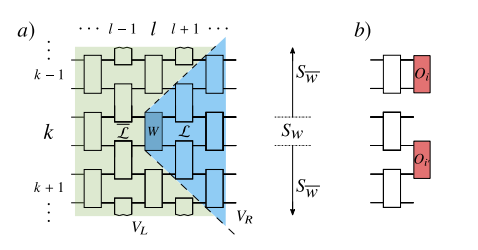
\includegraphics{LiteratureReview/Appendices/alterlayeransatz.png}
    \caption{
        Altering Layered Ansatz. 
        a) Each block $W_{kl}$ on $m$ qubits is parameterized.
        $S_k$ is the $m$ qubit subsystem on which $W_{kL}$ acts, note that L is the last layer of the ansatz $U(\theta)$.
        The right light-cone
    }
    \label{Altering Layered Ansatz}
\end{figure}

if a \almarginpar{Explain what is "local" vs "global" cost function}\underline{local cost} function is used, then there is a lower bound for the variants of the gradients that depends on the number of qubits and some configurations of the circuit. 
For a $L$-layered ansatz, let the variance $\mathrm{Var}[\partial_v C]$ of the partial derivative of the cost function $C$, the lower bound $G_n$ for the variance is:
\begin{equation}
    G_n(L,l) \leq \mathrm{Var}[\partial_k C]
\end{equation}
\begin{equation}
    G_n(L,l) = \frac{{2}^{m(l+1)-1}}{{({2}^{2m}-1)}^{2}{({2}^{m}+1)}^{L+l}}
    \times \mathop{\sum}\limits_{i\in {i}_{{\mathcal{L}}}}\mathop{\sum}\limits _{{(k,k^{\prime} )\in {k}_{{{\mathcal{L}}}_{\text{B}}}}\atop {k^{\prime} \geqslant k}}{c}_{i}^{2}\epsilon ({\rho }_{k,k^{\prime} })\epsilon ({\widehat{O}}_{i})\ ,
\end{equation}
Where the forward light-cone $\mathcal{L}$ is a set of gates with at least one input connected to the output of a block $W$; 
The backward light-cone $\mathcal{L}_\text{B}$ is a set of gates with at least one output connected to the input of block $W$;
$S_k$ is the $m$-qubit subsystem;
$i_{\mathcal{L}}$ is a set of indices such that the operators $\hat{O_i}$ act on qubits in $\mathcal{L}$;
$k_{\mathcal{L}_B}$ is a set of indices such that the subsystem $S_k$;

\almarginpar{What is $G_n$}If the total depth $L$ is in the range $O(\log(n))$ of the number of qubits (a shallow configuration), then the lower bound cannot vanish faster than $\Omega(1/\mathrm{poly}(n))$. 
Thus, no Barren Plateau occurs in this case.\almarginpar{You throw lots of formulas in but do not explain much}



\subsubsection{Layerwise learning for quantum neural networks}

There is another method that manipulates the circuit depth throughout the training period studied by Skolik et al. \cite{skolikLayerwiseLearningQuantum2021}. 
In more detail, the algorithm consists of two phases:

\almarginpar{Good find "qcircuit"!}\textbf{The first phase} constructs the ansatz by adding layers one by one, with the parameters are all initially zero. For a small number $s$ of starting layers, the set of parameters $\vec{\theta_1}$, and $W$ operators connecting qubits, then the initial layers $l_1(\vec{\theta_1})$ is presented:

\begin{equation}
    l_1(\vec{\theta_1})
    = \prod_{j=1}^s U_{1_j}(\vec{\theta_{1_j}}) W \;,
\end{equation}

Where each consecutive layer $l_i(\vec{\theta_i})$ of form
\begin{equation}
    l_i(\vec{\theta_i})
    =U_i(\vec{\theta_i}) W \;,
\end{equation}
is added after a certain number of epochs and the previous layers' parameters become fixed. 
One epoch is the set of iterations for the algorithm to see each training sample; an update of all trainable parameters is called one iteration.

This process can stop when a certain circuit depth is reached or until the objective function's value does not improve with additional layers.
Figure \ref{ll circuit} provides an illustrative example of the final circuit.
Eventually, we obtain the final circuit of $L$ layers:

\begin{equation}
    U(\vec{\theta})
    = \prod_{i=0}^L l_i (\vec{\theta_i}) \;.
\end{equation}
\begin{figure} 
    \centerline{
        \Qcircuit @C=1em @R=0em {
        & \multigate{4}{l_1(\vec{\theta_1})}    & \multigate{4}{l_2(\vec{\theta_2})}    & \qw &        & & \multigate{4}{l_i(\vec{\theta_i})}   & \qw\\
        & \ghost{l_1(\vec{\theta_1})}           & \ghost{l_2(\vec{\theta_2})}           & \qw &        & & \ghost{l_i(\vec{\theta_i})}          & \qw\\
        & \ghost{l_1(\vec{\theta_1})}           & \ghost{l_2(\vec{\theta_2})}           & \qw & \cdots & & \ghost{l_i(\vec{\theta_i})}          & \qw\\
        & \ghost{l_1(\vec{\theta_1})}           & \ghost{l_2(\vec{\theta_2})}           & \qw &        & & \ghost{l_i(\vec{\theta_i})}          & \qw\\
        & \ghost{l_1(\vec{\theta_1})}           & \ghost{l_2(\vec{\theta_2})}           & \qw &        & & \ghost{l_i(\vec{\theta_i})}          & \qw\\
        }
    }
    \caption{
        Constructing the ansatz from shallow layers.
    }\label{ll circuit}
\end{figure}


\textbf{The second phase} takes the pre-trained circuit from phase one and trains \almarginpar{What are these?}\underline{larger adjacent partitions} of layers at a time. 